\section{Empirical Data}


August - December 2020, the first semester on the master degree was spent finding a supervisor and deciding/ orienting on what I wanted to write about. The second semester was for the most part theoretical, getting to know the museum domain and working on the research question and angle for the thesis. Started 

\begin{figure}[h]
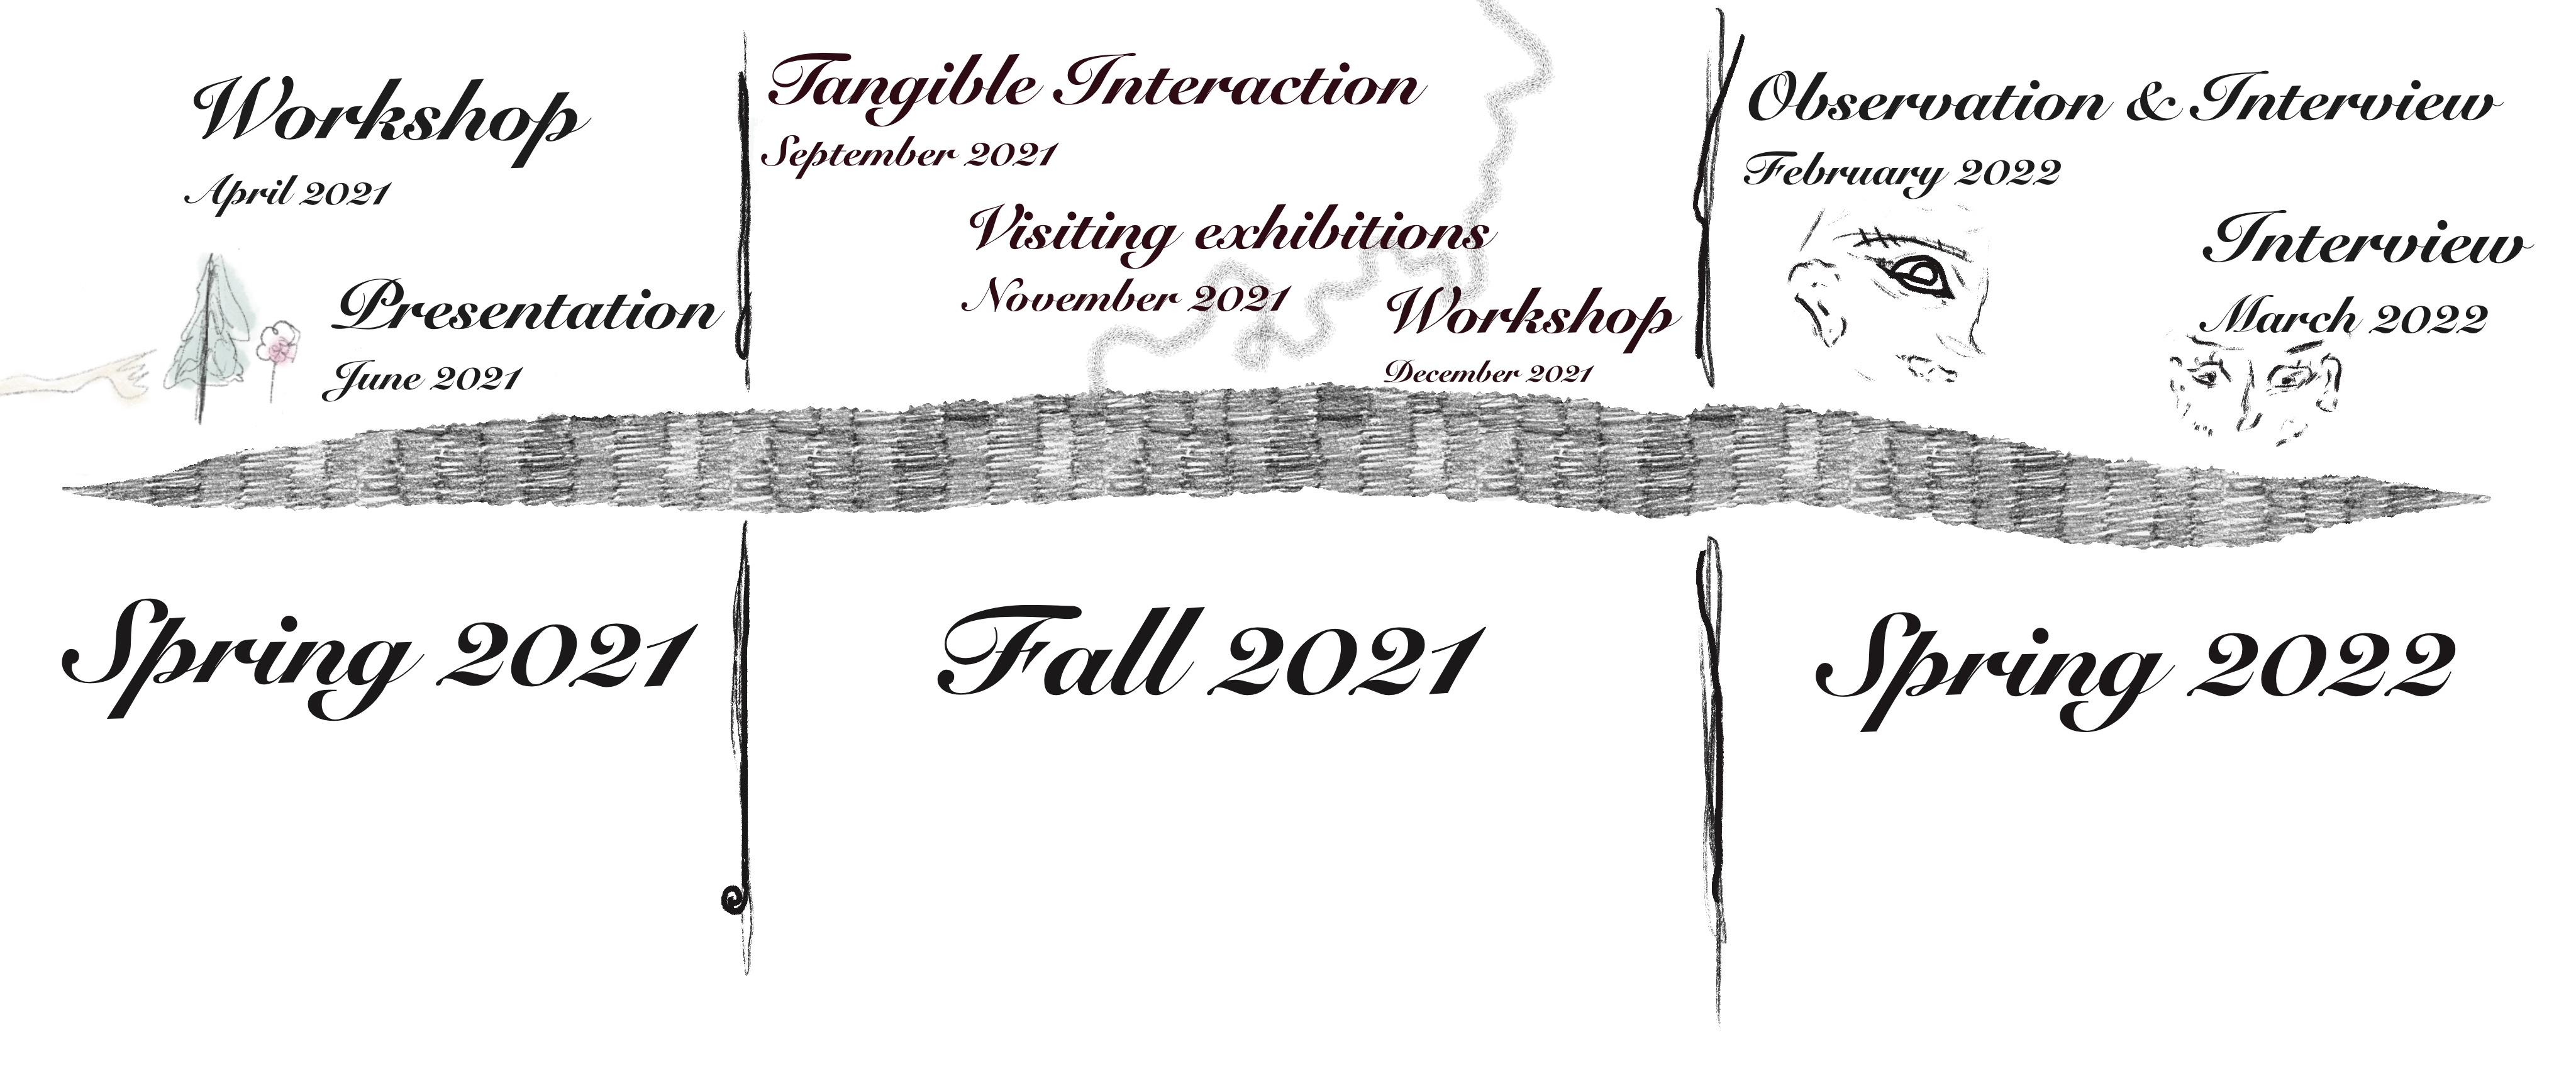
\includegraphics[width=13cm]{pictures/timeline.jpg}
\centering 
\end{figure}

The dataset that I/we have gathered for this thesis is as following:
- Workshop, april 21
- Presentation, june 21
- 4/5 exhibitions, fall 21
- Observation of school children in Klimahuset, february 22
- Interview and observation w/ concept developer at Munch, march 22

\section{Creating the theoretical framework}

Originating:
Positioning:
shaping:
shaped:

My question and aim for this thesis is to provide designers with a broader vocabulary for situations when they are working with a design project that touches the areas of interest in this paper; interactive meaning-making in a museum context. I have worked hard to obtain findings in this paper that are grounded in some practical way or aftermath where hands-on designers and others can gain practical knowledge and guidelines for when they are working with this. 


\section{The role of prototyping in this thesis}
Research through design is a type of research practise where the researcher create artefact- or object prototypes to gain the necessary insight needed to drive and conduct the research project. Prototyping, or the use of prototypes can be used in a variety of ways, and in every stage throughout the project. In the field of human-computer interaction (HCI), software engineering and design, the term prototype is commonly used to signify a specific kind of object used in the design process (Lim et. al., 2008, p. 2). The prototypes are either physical or digital, and function as either a speculative solution, as a manifestation of a design idea, or to explore a design space - all in relation to the research scope and focus. Prototypes are the means by which designers organically and evolutionary learn, discover, generate and refine designs \cite{lim_anatomy_2008, p.2}. They are design-thinking enablers deeply embedded and immersed in design practise, not just as tools for evaluating or proving successes or failures of design outcomes (Lim et. al., 2008, p. 2).

In the search for a new way of thinking about prototypes and prototyping, based on the need for exploring and establishing a definition that differs from current approaches in software engineering contexts where engineers use prototypes to identify or satisfy requirements: Lim et. al., conceptualise prototypes as tools for traversing a design space where all possible design alternatives and their rationales can be explored (Lim et. al., 2008, p. 2). In that way, the prototype serves as a communicative manifestation, where the designer is enabled to communicate the rationales of their design decisions through the prototype (Lim et. al., 2008, p. 2). Prototypes stimulate reflections, and designers use them to frame, refine and discover possibilities in a design space (Lim et. al., 2008, p. 2). This new way of thinking about prototypes differs markedly from requirement-oriented approaches like software engineering, recognising design activities as flexible rather than rigid, reflective rather than prescriptive, and problem-setting rather than problem-solving (Schön, 1982). A design idea that satisfies all the identified requirements does not guarantee that it is the best design since a number of ways can meet each requirement (Lim et. al., 2008, p. 2). If the focus of prototyping is framing and exploring a design space, what matters is not identifying or satisfying requirements using prototypes but finding the manifestation that in its simplest form, filters the qualities in which designers are interested, without distorting the understanding of the whole (Lim et. al., 2008, p. 2). In order to support this perspective and to provide a stable foundation for the study of prototypes in HCI, Lim et. al. (2008) proposes a framework for conceptualising prototypes. The framework is an attempt to create an understanding of the nature of prototypes in general and to provide a language for articulating the characteristics of a particular prototype (Lim et. al., 2008, p. 3). Two fundamental aspects of prototyping form the basis of the framework:

1) prototypes are for traversing a design space, leading to the creation of meaningful knowledge about the final design as envisioned in the process of design, and
2) prototypes are purposefully formed manifestations of design ideas.
(Lim et. al., 2008, p. 3)

Will answer these:
What values are important in my context?
What is my design outcomes?
What is my design space?
Experience prototyping? Am I going to prototype an experience?
Why and how do I intend a particular prototype to support the design process?

In this thesis, the role of prototyping will be a proof of concept where the perspectives are manifested or represented. As a proof of concept of how I have used the framework/ thinking to design a meaningful interactive experience.
The prototypes main function is to work as a “mediator”, to facilitate for conversations with museumspeople or designer that will give insight to what the prototypes adresses.
